
\renewcommand{\algorithmicrequire}{\textbf{Input: }}
\renewcommand{\algorithmicensure}{\textbf{Output: }}

\section{Louvain \textit{Method}}

Deteção de uma comunidade de um grafo envolve a partição deste em comunidades de nós densamente conectados. A modularidade mede a densidade das arestas dentro das comunidades em comparação com aquelas entre comunidades e é usada para saber a qualidade da partição de um grafo em comunidades criadas por um algoritmo. 

\subsubsection{Modularidade}

Modularidade de uma partição para grafos com pesos nas arestas:

\begin{equation}
Q = \frac{1}{2m} \sum_{i,j} [ A_{ij} - \frac{k_i k_j}{2m} ] \delta(c_i ,c_j)
\label{eq:MN}
\end{equation}


\begin{itemize}
	\item $A_{ij}$ é o peso da aresta entre $i$ e $j$.
	\item $k_i = \sum_j A_{ij}$ é a soma do peso de todas as arestas de $i$, com o mesmo significado para $k_j$.
	\item $c_i$ é a comunidade de $i$, com o mesmo significado para $c_j$.
	\item $\delta(c_i,c_j)$ é a igualdade entre $c_i$ e $c_j$ ( os dois vértices serem da mesma comunidade).
	\item $m = \frac{1}{2}\sum_{ij} A_{ij}$ é a soma do peso de todas as arestas %metade porque consideram que 
%o peso das arestas será calculado duas vezes, por cada vértice. Logo é necessário dividir.
\end{itemize}




\subsection{Algoritmo de Louvain \textit{Method}}
Algoritmos existentes para cálculo de modularidade em grafos são muito pouco eficientes para grafos de larga escala e é também necessário detetar as comunidades dentro de comunidades (sub-comunidades). Para isto em \cite{louvainDoc} foi proposto um novo algoritmo.

As suas duas fases são:

\paragraph{Primeira}
Todos os vértices têm uma comunidade diferente, sendo que existem N comunidades onde N é o número de vértices.
Para cada nó é visto os seus adjacentes e calculado o ganho de modularidade que existiria se o nó fosse adicionado à comunidade do vizinho. Sendo adicionado à comunidade do vizinho com o maior ganho não negativo. Esta fase continua até já não existir ganhos (modularidade máxima).
O ganho obtido movendo um nó isolado $i$ para uma comunidade $C$ é calculado através da equação:


\begin{equation}
\label{eq:GND}
 \Delta Q  =  [\frac{\sum_{in} + k_{i,in}}{2m} - (\frac{\sum_{tot} +k_i}{2m})^2] - [\frac{\sum_{in}}{2m} - (\frac{\sum_{tot}}{2m})^2 - (\frac{k_i}{2m})^2] 
\end{equation}

\begin{itemize}
	\item $\sum_{in}$ é a soma do peso de todas as arestas dentro de $C$ (vão de um vértice em C para outro)
	\item $\sum_{tot}$ é a soma do peso de todas as arestas dos vértices de $C$. %( inclui Ein ou é aqueles que vão de outros vértices para os da comunidade C?)
	\item $K_i$ é a soma do peso de todas as arestas de $i$. %(incidentes...)
	\item $K_{i,in}$ é a soma do peso de todas as arestas de $i$ para vértices de $C$.
	\item $m$ é soma de do peso total do grafo.
\end{itemize}

\paragraph{Segunda}
É criado um novo grafo cujo vértices sejam as comunidades anteriormente encontradas e o peso da aresta entre duas comunidades é calculado somando o peso de todas as arestas entre estas. É depois aplicada novamente a 1ª fase a este novo grafo.
Estas duas fases são nomeadas 'passos' e continuam até ser encontrada a modularidade máxima.


É assim apresentado o seguinte algoritmo onde \verb|i| representa um vértice, \verb|comm| uma comunidade, \verb|comm[i]| a comunidade de \verb|i|, \verb|tot[comm]| representa $E_{tot}$ para a comunidade \verb|comm| e \verb|m2| é $2m$.
\begin{algorithm}
\caption{Primeiro passo}
\label{alg:LMPS}

	\algorithmicrequire{Grafo G}
	\begin{enumerate}
		\item Para todos os vértices $i$ em $G$ $comm[i] \gets i$
		\label{SS1}
		\item Remover $i$ da sua comunidade atual $comm[i]$
		\item Para todos os vizinhos $j$ de $i$ $comm \gets comm[j]$ e computar o ganho conseguido em mover $i$ para $comm$ $curr\_gain \gets computeGain(i,comm,m2)$
		\item Inserir $i$ na comunidade com o maior ganho atualizando o $tot[comm]$ de acordo.
		\item Se algum $i$ foi movido para uma comunidade diferente então voltar para ~\ref{SS1}.
		\item Iniciar o segundo passo especificado no algoritmo~\ref{alg:louvainPasso2}.
	\end{enumerate}
\end{algorithm}


Neste algoritmo $computeGain$ calcula o ganho usando a equação referida em cima.

\begin{algorithm}
\caption{Segundo passo}
\label{alg:louvainPasso2}
	\begin{enumerate}
		\item Se ocorreu alguma mudança de comunidade no passo anterior
		\item Passar todos os vértices $i$ na mesma comunidade para uma só comunidade
		\item O peso das arestas entre duas comunidades passa a ser a soma do peso das arestas dos nós entre duas comunidades e as arestas para a mesma comunidade passam a ser nós circulares
		\item Voltar a executar o algoritmo \ref{alg:LMPS} com o novo grafo formado.
	\end{enumerate}
\end{algorithm}

O exemplo seguinte tem um total de 25 arestas, sendo que o seu \verb|m2| será 50:
\begin{figure}
\centering
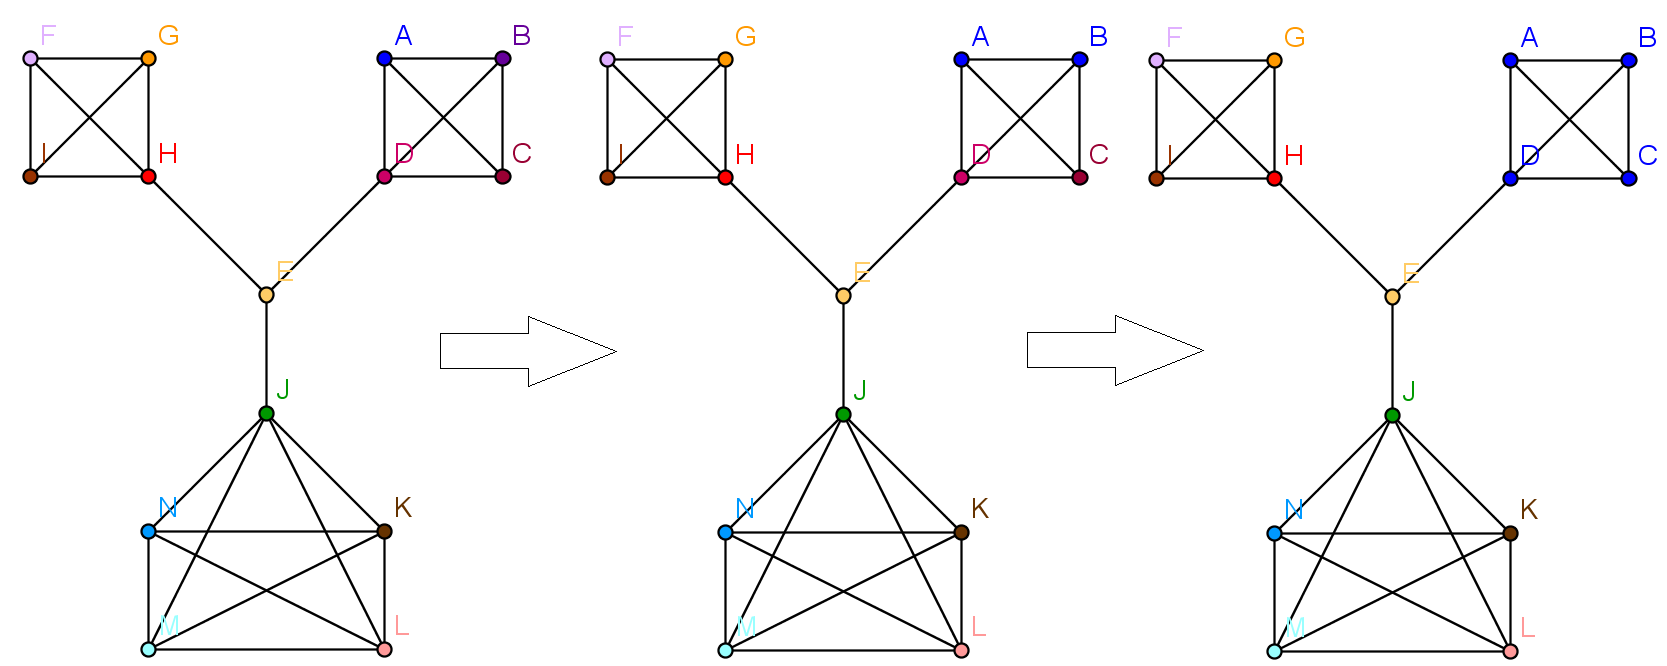
\includegraphics[width=90mm]{graphf1}
\caption*{Todas os vértices começam por pôr a sua comunidade igual ao seu id. De seguida, são removidos da comunidade atual e é calculado o ganho em inserir-los na comunidade de uns dos vizinhos, sendo posto na comunidade com o maior ganho.}
\end{figure}
\begin{figure}
\centering
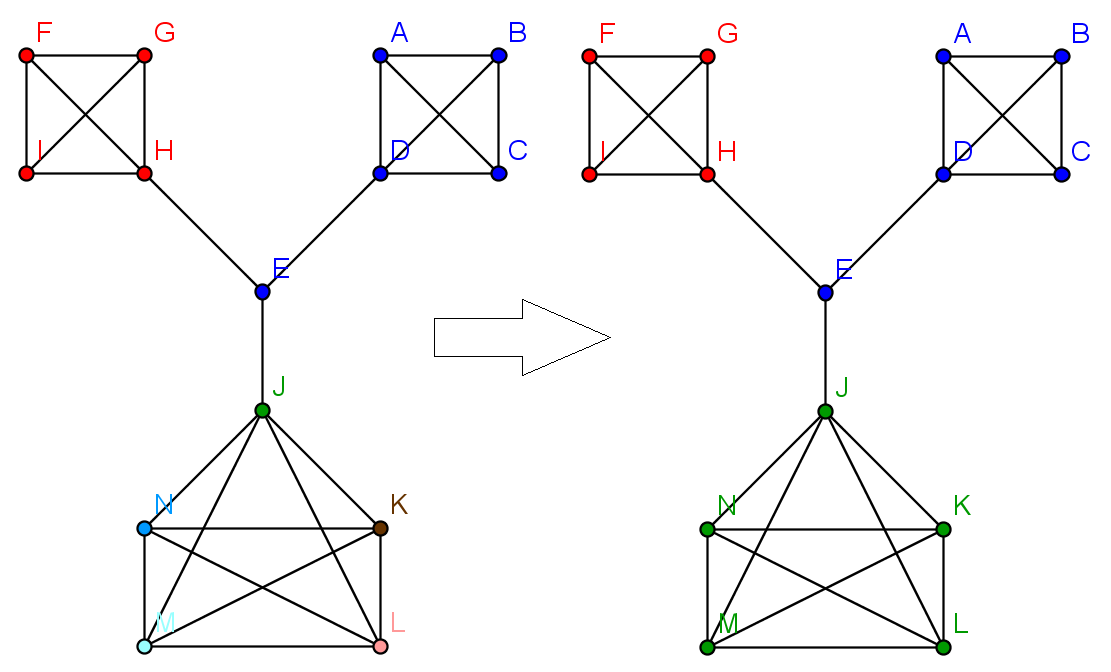
\includegraphics[width=90mm]{graphf2}
\caption*{Este processo continua até nenhuma vértice mover de comunidade.}
\end{figure}
\begin{figure}
\centering
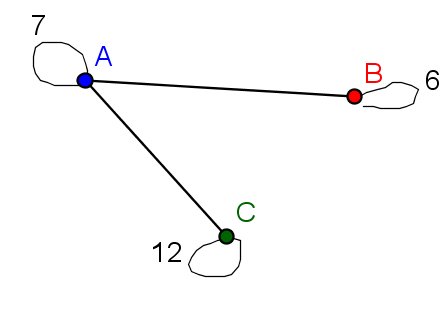
\includegraphics[width=60mm]{graphf3}
\caption*{No segundo passo as comunidades existentes passam a só um grafo e as arestas dentro da comunidade passam a ser uma única circular. É depois executado o primeiro passo mas neste exemplo já não ocorrem alterações.}
\end{figure}


\newpage
\subsection{Algoritmo de Louvain \textit{Method} Distribuído}
O método apresentado anteriormente pode ser usado para grafos de larga escala, mas o tamanho do grafo está limitado pela memória disponível na máquina.

É possível resolver a equação \ref{eq:GND} e obter a equação~\ref{eq:GD}.
\begin{equation}
	\Delta Q  =  K_{i,in} - \frac{\sum_{tot} K_i}{2m}
\label{eq:GD}
\end{equation}


Esta nova equação depende de menos variáveis e, visto que $K_{i,in}$ e $K_i$ são referentes a um único vértice, leva a que seja necessário trocar menos informação entre os vários vértices na versão distribuída deste método.

Cada vértice tem como valor:
\begin{itemize}
	\item \verb|id| o seu identificador único.
	\item \verb|deg| A soma do grau de todas as suas arestas. ($K_i$).
	\item \verb|tot| O total da soma dos graus das arestas incidentes aos vértices da sua comunidade. ($\sum_{tot}$).
	\item \verb|hub| O id do concentrador da sua comunidade.
\end{itemize}

O primeiro passo do algoritmo de Louvain \textit{Method}, presente em~\ref{alg:lmdPasso1} foi dividido em inicialização e 3 fases que se repetem até for atingido a modularidade máxima, sendo que uma iteração é uma passagem destas 3 fases.

\begin{algorithm}
\begin{minipage}{\textwidth}
\caption{Louvain \textit{Method} Distribuido Passo 1}
\label{alg:lmdPasso1}
\begin{enumerate}
  \item Inicialização
			\begin{enumerate}
				\item O \verb|hub| de todos os vértices passa a ser o \verb|id| do próprio vértice e \verb|tot| 				recebe \verb|deg|
			\end{enumerate}
	\item Primeira Fase
	\begin{enumerate}
	\item Se não for a primeira vez que está na primeira fase o vértice deve substituir o seu \verb|tot| e \verb|hub| por aqueles recebidos na mensagem
	\item Vértice envia aos seus adjacentes o seu \verb|id|, \verb|tot|, \verb|hub| e custo da aresta que o liga ao adjacente\footnote{Se as arestas não tiverem custo o custo considerado é 1}.
	\end{enumerate}
	
  \item Segunda Fase -  Ao receber uma mensagem o vértice deve:
  
		\begin{enumerate}
				\item Se não for a primeira vez que está na segunda fase o vértice deve verificar se nenhum vértice mudou de comunidade na segunda fase anterior e
						\subitem Se não for a primeira vez que está no primeiro passo e nunca ocorreram mudanças em nenhumas das segundas fases deste passo deve parar o algoritmo
						\subitem Caso contrário, deve começar o segundo passo descrito no algoritmo~\ref{alg:lmdPasso2}
				\item Calcular a melhor comunidade utilizando a equação~\ref{eq:GD}\footnote{Quando se calcula se a comunidade atual é a melhor comunidade é necessário remover o \textit{deg} atual do \textit{tot} da comunidade e, se o \textit{tot} passar a ser 0 então o ganho de modularidade será 0 de modo a impedir que os vértices nunca mudem de comunidade}. 
				Em caso de empate	escolher a comunidade em que \verb|hub| seja o menor.
				\label{prt:force}
				\item Em iteração pares o vértice não move para comunidades cujo \verb|hub| seja menor que o seu \verb|hub| atual.
				\item Registar globalmente se mudou de comunidade
				\item Atualizar \verb|hub| com o \verb|hub| da melhor comunidade e enviar para o \verb|hub| uma mensagem contendo \verb|id| e \verb|deg|.
		\end{enumerate}
		
  \item Terceira Fase - Os vértices, ao receberem as mensagens, devem:
\begin{enumerate}
		\item Se for uma iteração par:
				\subitem Calcular um novo \verb|tot| a partir dos \verb|deg| recebidos.
				\label{prt:cycle2}
				\subitem Se não pertencer a comunidade que está agregar escolhe como \verb|hub| o vértice da comunidade com o menor \verb|id|, caso contrário mantêm-se como \verb|hub|.
				\subitem Enviar uma mensagem a todos os elementos da comunidade que agregou com o novo \verb|tot| da comunidade.
		\item Se for uma iteração ímpar:
		\label{prt:cycle1}
		\subitem Se receber uma mensagem, não enviada pelo próprio vértice, em que o \verb|id| proveniente da mensagem seja igual ao \verb|hub| escolhido e o \verb|id| do vértice atual for maior que o \verb|id| proveniente da mensagem o vértice deve:
				\subsubitem Adicionar ao \verb|tot| atual o seu próprio \verb|deb|
				\subsubitem Registar que terá que enviar a si própria uma mensagem de atualização
				\subsubitem Escolhe a si próprio como \verb|hub|
		\subitem Enviar uma mensagem a todos os elementos da comunidade que agregou com o novo \verb|tot| da comunidade. Enviando a si mesmo caso tiver registado anteriormente.
\end{enumerate}
\end{enumerate}

	\end{minipage}
\end{algorithm}

No algoritmo~\ref{alg:lmdPasso1} os pontos~\ref{prt:force}~e~\ref{prt:cycle1} servem para tratar de possíveis ciclos que ocorrem quando dois \verb|hub| tentam mudar para a comunidade do outro.
Em iterações pares, no ponto~\ref{prt:force} um vértice é impedido de mudar de comunidade, efetivamente eliminando ciclos.
Mas em iterações ímpares o ponto~\ref{prt:force} não impede mudanças sendo que o ponto~\ref{prt:cycle1} trata de resolver os ciclos nestas iterações escolhendo o vértice de maior \verb|id| como representante.

Usar estas duas formas de resolução de ciclos e reeleger o \verb|hub| como está a ser feito no ponto~\ref{prt:cycle2} servem para aproximar as comunidades conseguidas por este algoritmo das comunidades conseguidas pelo algoritmo original reduzindo e aumentando o número de mudanças de comunidade dinamicamente.
%É de notar que, terceira fase, tanto no ponto~\ref{prt:cycle2}, no caso do vértice receber uma mensagem do \verb|hub| que ele elegeu na fase anterior, e no ponto~\ref{prt:same} o vértice não recebe uma mensagem de si próprio sendo que este, em~\ref{prt:cycle2}, tem que garantir que envia uma mensagem de atualização a si próprio e em~\ref{prt:same} um outro vértice irá enviar-lo a mensagem de atualização. Sendo que estes dois casos nunca ocorrem em simultâneo.

\paragraph{}
O segundo passo, presente em~\ref{alg:lmdPasso2} assenta sobre o primeiro, tendo apenas duas fases, que sobrepõem a segunda e terceira fase do primeiro passo.

\begin{algorithm}
\caption{Louvain \textit{Method} Distribuído Passo 2}
\label{alg:lmdPasso2}
\begin{enumerate}
	\item Primeira Fase
	
	\begin{enumerate}
		\item O vértice cria uma estrutura de tuplos (\verb|hub|,\verb|deg_s|), onde para cada comunidade presente nas mensagens recebidas, \verb|deg_s| será a soma de todos os \verb|deg| dos elementos dessa comunidade conhecidos através destas mensagens.
		\item Os vértices removem as suas arestas e enviam esta estrutura ao concentrador.
	\end{enumerate}
	
	\item Segunda Fase
	
	
	\begin{enumerate}
		\item O concentrador, com uma estrutura similar à da primeira fase agrega os valores de todos os elementos da comunidade.
		\item Para cada elemento da estrutura o concentrador deve criar novas arestas em que o \verb|id| de destino é o \verb|hub| do elemento e o peso da aresta é \verb|deg_s|, atualizando o seu \verb|deg|. Envia a si próprio uma mensagem com um \verb|tot| igual ao \verb|deg| agora calculado. Nota que o peso total de arestas é alterado neste ponto e deve ser atualizado.
		\item Recomeçar o passo 1.
	\end{enumerate}
\end{enumerate}
\end{algorithm}

Esta versão distribuída tenta criar comunidades aproximadas às das criadas pela versão não distribuída mas as comunidades formadas dependem das permutações realizadas não estando garantido que as comunidades formadas serão sempre as mesmas.

\paragraph{}
Existe uma versão distribuída deste algoritmo~\cite{disLM} que usa uma ideia parecida de dividir o algoritmo em 3 fase mas devido a diferença na forma de que os ciclos são resolvidos as comunidades formadas serão diferentes das comunidades formadas pelo nosso algoritmo, sendo que as formadas pelo nosso aproximam-se mais daquelas formadas pelo algoritmo de Louvain original. O nosso algoritmo tem também um número menor de \textit{supersteps} no primeiro passo, sendo que o algoritmo em~\cite{disLM} usa o Map Reduce do Hadoop para realizar o segundo passo.
Possivelmente serão feitos testes comparando o tempo de computação dos dois algoritmos.

O exemplo seguinte mostra o resultado da execução do algoritmo distribuído sobre o grafo anterior.

\begin{figure}[h]
\centering
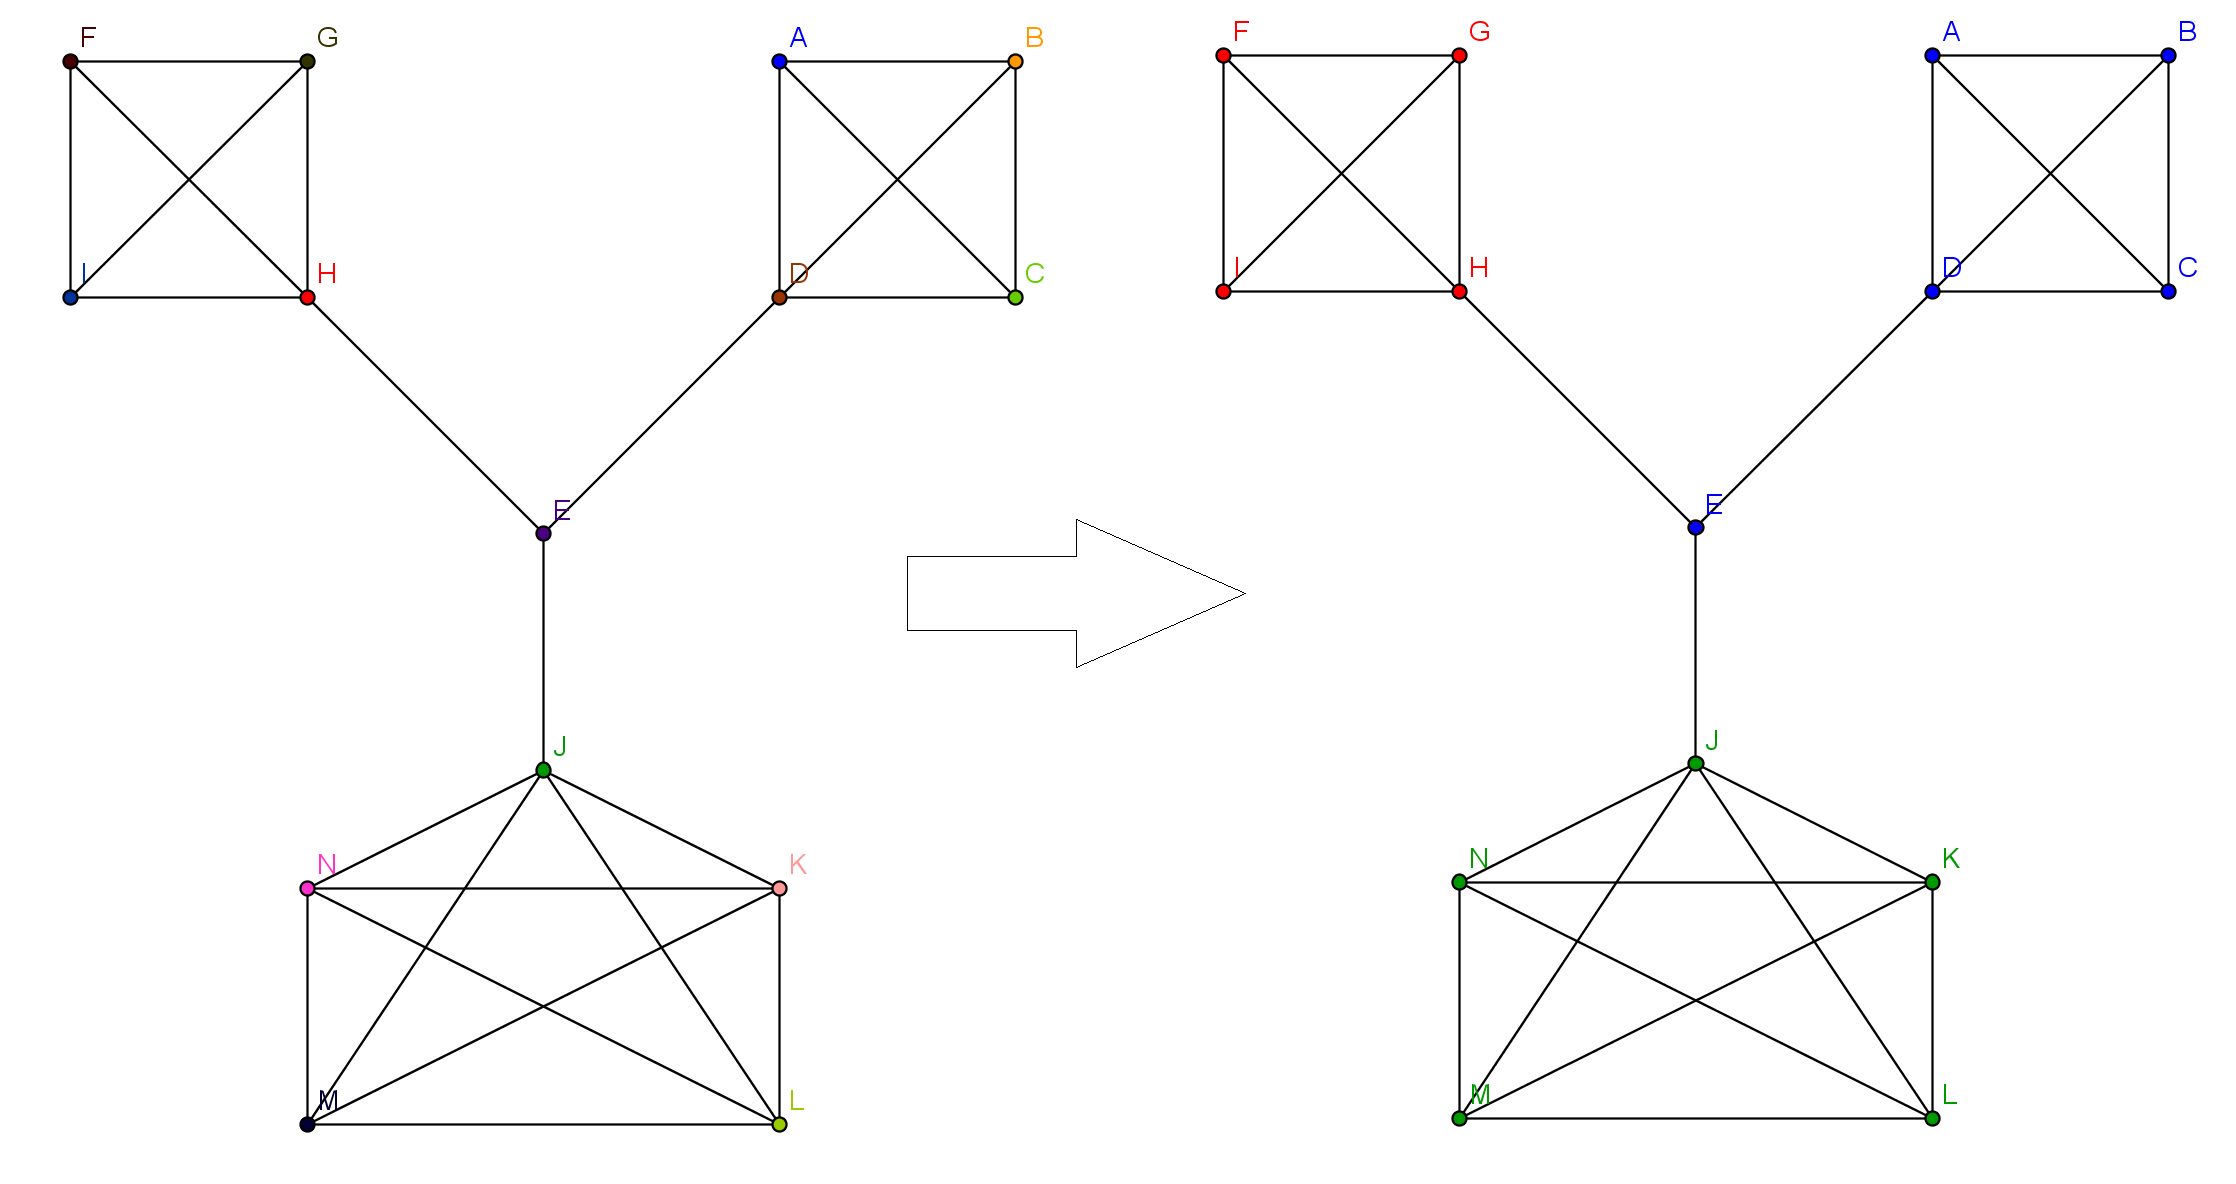
\includegraphics[width=90mm]{graphd1}
\caption*{Os vértices começam por decidir que serão o seu próprio $hub$. Depois começam por calcular a melhor comunidade mudando-se para tal. Como o algoritmo é distribuído existem várias mudanças em simultâneo}
\end{figure}
\begin{figure}[h]
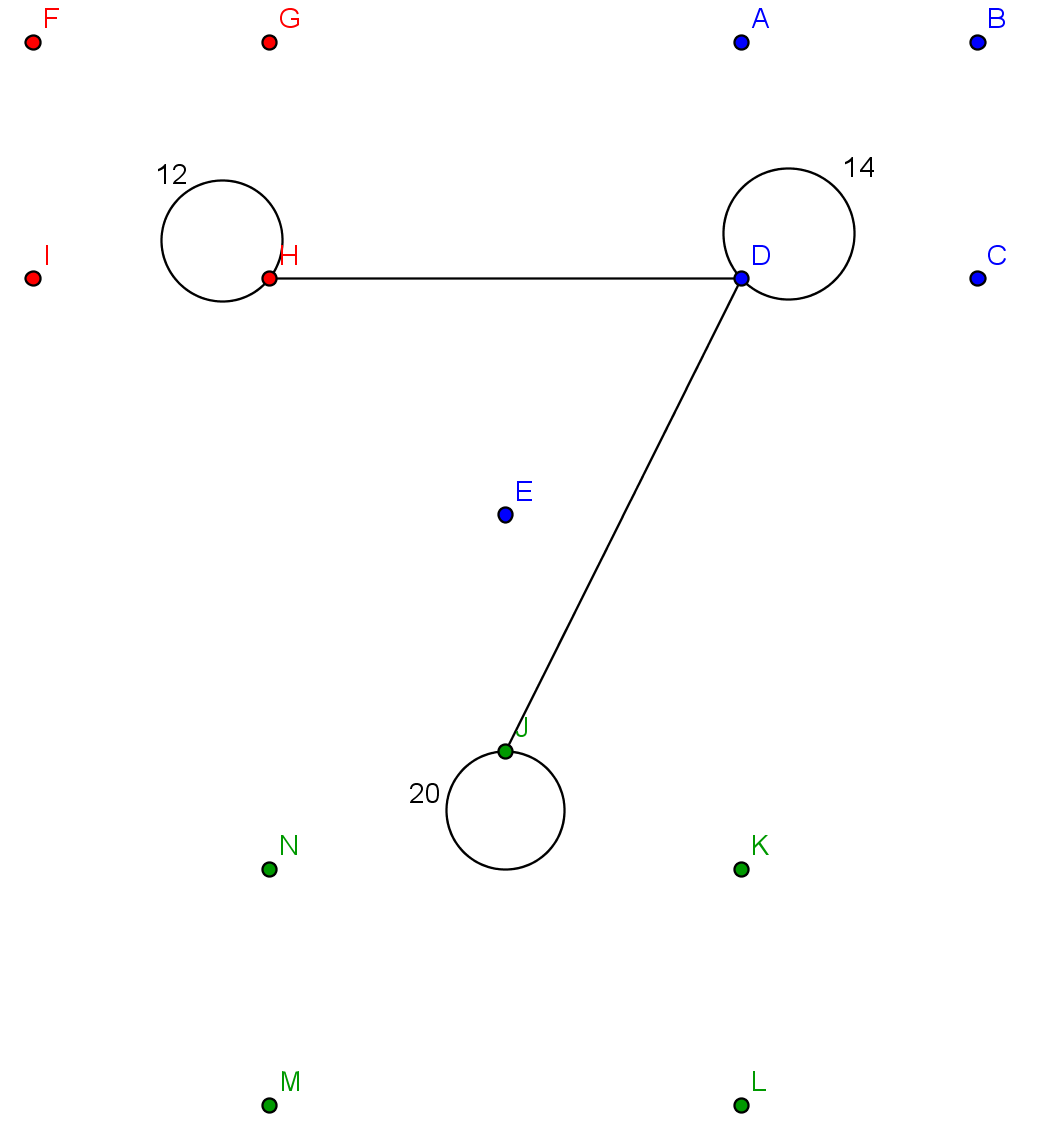
\includegraphics[width=90mm]{graphd2}
\caption*{No segundo passo os vértices removem as suas arestas e os representantes criam novas baseadas nas anteriores ligações entre os vértices das comunidades. Voltando ao primeiro passo onde já não ocorrem mudanças}
\end{figure}